\documentclass[main.tex]{subfiles}

\pagestyle{fancy}
\fancyhf{}
\fancyhead[LE]{\makebox[\pageoffset][l]{\bfseries\thepage}\bfseries\leftmark}
\fancyhead[RO]{\bfseries\rightmark\makebox[\pageoffset][r]{\bfseries\thepage}}

\begin{document}

\section*{Goal}
For our final experiment we will study calorimetry, a topic found in thermal physics which is another branch of physics. 

\section*{Equipment}
\begin{itemize}
\item
Styrofoam calorimeters
\item
Thermometer
\item
Triple-beam balance
\item
Copper, lead, and aluminium samples
\item
Water ice
\end{itemize}•

\section*{Theory}
The amount of energy required to raise the temperature of a sample by one degree Celsius (or equivalently one Kelvin) without causing a change of phase is called the heat capacity of that substance. The heat capacity per unit mass is called the specific heat of the substance. Historically, the amount of heat required to raise the temperature of one gram of water from $14.5\celsius$ to $15.5\celsius$ was defined to be 1 calorie, which in SI units is equivalent to 4.186 J. The Calorie that is used in food labeling is 1000 calories or 4186 J. In order to measure this quantity we will use the conservation of energy also known as the first law of thermodynamics,
\begin{equation}
\Delta U=W+Q,
\end{equation}
where $\Delta U$ is the increase in total internal energy of a closed system, $W$ is the work done on the system and $Q$ is the heat added to the system. When there is no work done on the system, such as the assumption of our experiment then the change in energy is equal to the heat added to the system alone. The heat added to a system of mass $m$ in terms of specific heat $c$ and temperature $T$ is,
\begin{equation} \label{eq:Heat}
Q=mc\Delta T.
\end{equation}
As we will be placing hot metal samples in relatively cool water, the heat will transfer from the metal sample into the water since heat always tends to flow from a hotter to a cooler body. We can describe this by the following equation,
\begin{equation} \label{eq:Metal}
Q = m_{w}c_{w}\Delta T_{w}+m_{m}c_{m}\Delta T_{m}=0,
\end{equation}
in which the first term describes the heat added to the water and the second term describes that of the metal sample. Using Equation~\eqref{eq:Metal} we can then determine the specific heat of our metal sample given that we know all other data.

\begin{wrapfigure}{r}{0.5\textwidth}
\centering
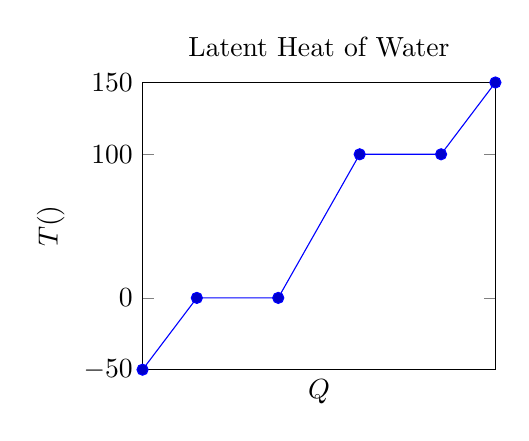
\begin{tikzpicture}
\begin{axis}[
	title={Latent Heat of Water},
	xlabel=$Q$, ylabel=$T (\celsius)$,
	ytick={-50,0,100,150}, xtick=\empty,
	xmin=0, xmax=3.25, 
	ymin=-50, ymax=150,
	width=0.5\textwidth
]
\addplot coordinates {
	(0,-50)
	(.5,0)
	(1.25,0)
	(2,100)
	(2.75,100)
	(3.25,150)
};
\end{axis}
\end{tikzpicture}
\caption{} \label{fig:Latent}
\end{wrapfigure}
In the second part of the experiment, we will melt ice in liquid water. If we were to graph the temperature of the ice versus the amount of heat put into the system we would see a graph similar to Figure~\ref{fig:Latent}. Most notable are the segments of Figure~\ref{fig:Latent} at the melting/freezing ($0\celsius$) and boiling/condensation ($100\celsius$) points as the graph reaches plateaus at both these points. As the temperature doesn't change in these regions, Equation~\eqref{eq:Heat} becomes nonsensical therefore we need a different expression to describe the heat transfer in the system. We handle this problem by introducing a constant known as the \emph{latent heat} which describes the energy that is being absorbed or released during one of these transitions. The latent heat of fusion, the constant for melting/freezing, denoted by $L_f$ is related to the heat by,
\begin{equation}
Q=mL_f
\end{equation}
The ice and water can be regarded as a ``closed" system, i.e., they do not exchange any energy with the lab because they are contained within a rigid, well-insulated calorimeter, a vessel for measuring heat flows. Hence there should be zero net heat flow, $Q=0,$ for the water-ice system. The ice (mass $m_i$) starts out (in a warm lab) on the verge of melting, so we can assume its initial temperature is $0\celsius.$ When we put it in the calorimeter with warm water (mass $m_w$), the ice melts at $0\celsius (Q_1=m_i L_f),$ then heats up by an additional temperature change $\Delta T_i (Q_2=m_i c_w \Delta T_i).$ Note that in this second term we use the specific heat of water ($c_w=4186 \text{ J}/\text{kg}\celsius$), not that of solid ice ($c_i=2093 \text{ J}/\text{kg}\celsius$) because the ice is now in the form of liquid melt water. The mass of this melt water is the same as that of the original ice ($m_i$), so even though it mixes with the warm water already in the calorimeter, we can identify the total heat it absorbs with help of the mass $m_i.$ Finally, we must include the heat transfer to the warm water as it cools down ($Q_3=m_w c_w \Delta T_w<0$). Adding these three heats,
\begin{equation} \label{eq:Ice}
Q=m_i L_f+m_i c_w \Delta T_i+m_w c_w \Delta T_w=0.
\end{equation}
Using Equation~\eqref{eq:Ice} we can then solve for the latent heat.

\section{Setup I: Specific Heat of a Metal}

\subsection*{Procedure}
\begin{enumerate}
\item \label{step:metal_start}
Record all masses in kilograms. Determine the mass of the calorimeter, thermometer, and stirring rod.
\item
Fill the calorimeter about $^2\!/_3$ full of water from the tap in the room.
\item
Determine the mass of the water by obtaining the mass of the entire system of calorimeter, water, rod, and thermometer. The calorimeter, rod, and thermometer take very little heat so we can consider them to be negligible to the thermodynamic process.
\item
At the lecture desk have the instructor place a hot metal sample carefully into the calorimeter and record the initial temperature of the sample.
\item
Use the stirring rod to keep the water circulated so the heat will be evenly distributed. Read the temperature at one minute intervals until the system comes to its equilibrium temperature i.e., when the temperature stops changing.
\item \label{step:metal_end}
Determine the mass of the system with the sample added to find the mass of the sample.
\item
Bring the sample back to the lecture desk, empty the calorimeter and get fresh water then repeat steps~\ref{step:metal_start}--\ref{step:metal_end} for another sample of a different type.
\end{enumerate}•

\section{Setup II: Latent Heat of Fusion}
\begin{enumerate}
\item
Repeat the above procedure except use a small chunk of ice cubes instead of the metal sample. Make sure to dry the ice with a paper towel before placing it into the calorimeter.
\end{enumerate}•

\section*{Analysis}
\begin{enumerate}
\item
Use Equation~\eqref{eq:Metal} to calculate the specific heat of the two metal samples. Compare with the standard value of the sample. The standard values are as follows:
\[
c_{\text{Pb}}=128 \text{ J}/\text{kg}\celsius, \qquad c_{\text{Al}}=900 \text{ J}/\text{kg}\celsius, \qquad c_{\text{Cu}}=387 \text{ J}/\text{kg}\celsius.
\]
\item
Use Equation~\eqref{eq:Ice} to calculate the latent heat of fusion for water. Compare with the standard value of $3.33\e5 \text{ J}/\text{kg}.$
\end{enumerate}

\begin{samepage}
\hrulefill \\
\emph{Chapter~\ref{chap:Calorimetry}:} \textbf{Calorimetry}
\begin{enumerate}
\item
\textbf{(50)} Complete the following data worksheet displaying sample calculations for all analysis items. 
\end{enumerate}•
\end{samepage}

\newpage
\enlargethispage{3cm}
\section{Calorimetry Data Sheet}

\begin{onehalfspace}
Name:\rule[-1mm]{4cm}{.1pt}\\
Attach a sheet to this one with all calculations on it (or use the back of this sheet).
\subsection*{Setup I}
\begin{wraptable}{r}{0.25\textwidth}
\begin{tabular}{|c|c|}
\hline
\multicolumn{2}{|c|}{Metal 1}\\
\hline
Time (min) & Temperature ($\celsius$)\\
\hline
0 & \\
\hline
1 & \\
\hline
2 & \\
\hline
3 & \\
\hline
4 & \\
\hline
5 & \\
\hline
6 & \\
\hline
7 & \\
\hline
\end{tabular}•
\end{wraptable}
\begin{tabular}{cccc}
Metal 1: & Copper & Lead & Aluminium
\end{tabular}\\
Mass of cup, thermometer, stir rod, and lid:\rule[-1mm]{2cm}{.1pt}\\
With water:\rule[-1mm]{2cm}{.1pt} Mass of water $(m_w)$:\rule[-1mm]{1.7cm}{.1pt}\\ \\
Initial temperature of sample $(T_{i,m})$:\rule[-1mm]{2cm}{.1pt}\\
Mass of calorimeter assembly and sample:\rule[-1mm]{2cm}{.1pt}\\
Mass of sample $(m_m)$:\rule[-1mm]{2cm}{.1pt}\\ \\
Calculated specific heat $(c_m)$:\rule[-1mm]{2cm}{.1pt} $\text{J}/\text{kg}\celsius$\\
Percent error:\rule[-1mm]{2cm}{.1pt}\\

\begin{wraptable}{r}{0.25\textwidth}
\begin{tabular}{|c|c|}
\hline
\multicolumn{2}{|c|}{Metal 2}\\
\hline
Time (min) & Temperature ($\celsius$)\\
\hline
0 & \\
\hline
1 & \\
\hline
2 & \\
\hline
3 & \\
\hline
4 & \\
\hline
5 & \\
\hline
6 & \\
\hline
7 & \\
\hline
\end{tabular}•
\end{wraptable}
\begin{tabular}{cccc}
Metal 2: & Copper & Lead & Aluminium
\end{tabular}\\
Mass of cup, thermometer, stir rod, and lid:\rule[-1mm]{2cm}{.1pt}\\
With water:\rule[-1mm]{2cm}{.1pt} Mass of water $(m_w)$:\rule[-1mm]{1.7cm}{.1pt}\\ \\
Initial temperature of sample $(T_{i,m})$:\rule[-1mm]{2cm}{.1pt}\\
Mass of calorimeter assembly and sample:\rule[-1mm]{2cm}{.1pt}\\
Mass of sample $(m_m)$:\rule[-1mm]{2cm}{.1pt}\\ \\
Calculated specific heat $(c_m)$:\rule[-1mm]{2cm}{.1pt} $\text{J}/\text{kg}\celsius$\\
Percent error:\rule[-1mm]{2cm}{.1pt}\\
\subsection*{Setup II}
\begin{wraptable}{r}{0.25\textwidth}
\begin{tabular}{|c|c|}
\hline
\multicolumn{2}{|c|}{Ice Water}\\
\hline
Time (min) & Temperature ($\celsius$)\\
\hline
0 & \\
\hline
1 & \\
\hline
2 & \\
\hline
3 & \\
\hline
4 & \\
\hline
5 & \\
\hline
6 & \\
\hline
7 & \\
\hline
\end{tabular}•
\end{wraptable}
Mass of cup, thermometer, stir rod, and lid:\rule[-1mm]{2cm}{.1pt}\\
With water:\rule[-1mm]{2cm}{.1pt} Mass of water $(m_w)$:\rule[-1mm]{1.7cm}{.1pt}\\ \\
Initial temperature of ice: $T_{i,i}=0\celsius$\\
Mass of calorimeter assembly and sample:\rule[-1mm]{2cm}{.1pt}\\
Mass of ice $(m_i)$:\rule[-1mm]{2cm}{.1pt}\\ \\
Calculated latent heat $(L_f)$:\rule[-1mm]{2cm}{.1pt} J/kg\\
Percent error:\rule[-1mm]{2cm}{.1pt}
\end{onehalfspace}

\end{document}
